\documentclass[tikz, border=3mm]{standalone}
\usepackage{tikz}
\usetikzlibrary{arrows.meta, decorations.markings, angles, quotes, calc}

\begin{document}
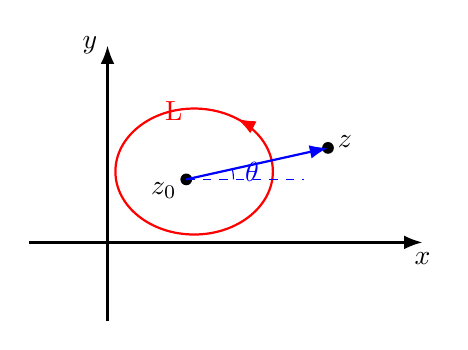
\begin{tikzpicture}[
    >=Latex, % Set default arrow tip style
    dot/.style={fill=black, circle, inner sep=1.5pt} % Style for points
]

% Axes
\draw[->, thick] (-1, 0) -- (4, 0) node[below] {$x$};
\draw[->, thick] (0, -1) -- (0, 2.5) node[left] {$y$};

% Define coordinates
\coordinate (z0) at (1, 0.8);
\coordinate (z)  at (2.8, 1.2); % Point on the curve
\coordinate (curve_center) at ($(z0)+(0.1,0.1)$); % Center ellipse near z0

% Define ellipse radii
\def\xrad{1.0}
\def\yrad{0.8}

% Draw the red closed curve L (ellipse) using explicit radius syntax
\draw[red, thick,
    postaction={decorate, decoration={markings, mark=at position 0.15 with {\arrow{>}}}} % Counter-clockwise arrow near top-left
] (curve_center) ellipse [x radius=\xrad, y radius=\yrad] % <<< FIX: Explicit syntax
    % Position label using 'pos' along the path
    node[red, above left, inner sep=1pt] at (1,1.5) {L}; % <<< FIX: Correct label positioning (0.375 is approx 135 deg)

% Draw points
\node[dot, label={[below left]$z_0$}] at (z0) {};
\node[dot, label={[right]$z$}] at (z) {};

% Draw vector from z0 to z
\draw[->, thick, blue] (z0) -- (z);

% Draw dashed horizontal line segment from z0
\coordinate (z0horz) at ($(z0)+(1.5,0)$); % Short horizontal segment
\draw[dashed, blue] (z0) -- (z0horz);

% Draw angle theta
\pic [draw, blue, angle radius=0.6cm, "$\theta$", angle eccentricity=1.4] {angle = z0horz--z0--z};

\end{tikzpicture}
\end{document}